\documentclass[]{article}

\usepackage[utf8]{inputenc}
\usepackage[russian]{babel}
\usepackage[left=1.5cm,right=1.5cm,top=2cm,bottom=2.5cm]{geometry}

\usepackage[fontsize=13pt]{scrextend}

% что-то за межстрочный интервал отвечающее
\renewcommand{\baselinestretch}{1.3}

\usepackage[nooneline]{caption}
\usepackage{subcaption}
\usepackage{indentfirst}
\usepackage{tabularx}
\usepackage{amsmath}
\usepackage{multirow}
\usepackage{hyperref}

\usepackage{booktabs, array} % для таблиц
%\usepackage[utf8]{inputenc}
%\usepackage[T2A]{fontenc}
%\usepackage[russian]{babel}

\usepackage{fancyhdr}


\setlength{\headheight}{15mm}


\usepackage[pdftex]{graphicx}
\graphicspath{{/home/maxim/Projects/Diploma/masters/text/img}}

%\pagestyle{fancy}
%\lhead{\textbf{\normalsize Проект 2}}
%\rhead{\textbf{\normalsize Выполнили: }\normalsize Кирякин %Максим, Куренкова Дарья, Коваль Наталия}



\begin{document}
	
	% \documentclass{report}
% \usepackage[russian]{babel}
% \usepackage[utf8]{inputenc}
% \usepackage[pdftex]{graphicx}

% \begin{document}

  \begin{titlepage}
  % ============== %
    \begin{center}
      
\includegraphics{img/msu_logo.jpg}
      \normalsize
      \\[0.1cm]
      Московский государственный университет имени М.В.Ломоносова
      \\[0.1cm]
      Факультет вычислительной математики и кибернетики
      \\[0.1cm]
      Кафедра исследования операций
      \\[1.5cm]
      {\Large Кирякин Максим Валерьевич}
      \\[1.0cm]
      \textbf{\Large Моделирование управления кредитным портфелем с учетом макроэкономических условий}
      \\[1.0cm]
      Курсовая работа
      \\[4.0cm]
      \begin{flushright}
      	\normalsize
         \textbf{Научный руководитель:}
         \\
         к.ф.м.н., Куренной Дмитрий Святославович
      \end{flushright}
      \vfill 
      Москва, 2025
    \end{center} 
  \end{titlepage}

% \end{document}

	
	\newpage
	\tableofcontents
	
	\newpage
	\section{Введение}
		
	
	Современный этап развития финансовых систем характеризуется возрастающей сложностью управления кредитными рисками на фоне динамичных макроэкономических изменений. Ускоренное внедрение технологий больших данных и машинного обучения, а также усиление глобальной экономической нестабильности, обусловленной санкционными ограничениями, пандемией и геополитическими кризисами, стимулируют трансформации подходов к управлению кредитными портфелями. В условиях турбулентности кредитные организации сталкиваются с необходимостью адаптации риск-менеджмента, включая модернизацию методов стресс-тестирования и разработку моделей, способных учитывать волатильность ключевых макроэкономических индикаторов. Данные факторы оказывают непосредственное влияние на вероятность дефолта заемщиков, что угрожает устойчивости финансовых институтов и требует разработки новых подходов к управлению кредитными портфелями.  
	
	Объектом настоящего исследования выступают кредитные портфели российских коммерческих банков, функционирующие в условиях высокой волатильности макроэкономической среды, включая колебания индекса РТС, ключевой ставки ЦБ РФ, курса рубля и динамики ВВП. Предмет исследования охватывает методы управления кредитными рисками, в частности, оценку кредитоспособности заемщиков, диверсификацию портфеля и прогнозирование вероятности дефолта (PD) с использованием количественных моделей, таких как модель Мертона. Последняя основанна на структурном подходе и формализует вероятность дефолта через соотношение стоимости активов компании \( V \), уровня долга \( D \) и волатильности доходности активов \( \sigma_V \):  
	
	\[
	PD = \Phi \left( \frac{\ln \left( \frac{V}{D} \right) + \left( r - \frac{\sigma_V^2}{2} \right) T}{\sigma_V \sqrt{T}} \right),  
	\]  
	
	где \( \Phi \) — функция распределения стандартной нормальной случайной величины, \( r \) — безрисковая ставка, \( T \) — временной горизонт.  
	
	В рамках работы были применены два подхода: теоритический и практический. Теоретический анализ базируется на изучении научных публикаций, нормативных документов и отчетов финансовых организаций, посвященных управлению кредитными рисками. Эмпирическая часть включает:  
	1) множественный регрессионный анализ для установления взаимосвязи между макроэкономическими индикаторами (инфляция, безработица, курс рубля) и параметрами модели Мертона;  
	2) расчет PD для российских компаний различных секторов экономики на основе данных финансовой отчетности (стоимость активов, долговая нагрузка, рыночная капитализация);  
	3) применение функций импульсного отклика для оценки влияния шоковых изменений макроэкономических переменных на вероятность дефолта.  
	
	Практическая часть исследования сфокусирована на анализе кредитного портфеля, сегментированного по отраслевому признаку. Для каждой компании рассчитаны параметры модели Мертона, включая волатильность активов и расстояние до дефолта, с последующей верификацией через регрессионные зависимости между этими параметрами и внешними макроэкономическими факторами. Установленные зависимости позволили расширить аналитический инструментарий за счет включения в модель дополнительных индикаторов, таких как курс валютной пары рубль-доллар, уровень инфляции и безработицы, что обеспечило более точную оценку устойчивости портфеля к внешним шокам.  
	
	Результаты работы демонстрируют значимость интеграции макроэкономических факторов в модели управления кредитным риском. Разработанный подход, сочетающий структурное моделирование и эконометрический анализ, позволяет не только прогнозировать PD в условиях нестабильности, но и формировать адаптивные стратегии диверсификации портфеля, минимизирующие потери в периоды кризисов. Полученные выводы имеют практическую ценность для российских банков, сталкивающихся с необходимостью балансирования между доходностью и риск-менеджментом в контексте санкционного давления и трансформации глобальных рынков.
	
	
	
	\section{Анализ современных методов управления кредитным риском}
	
	Кредитный риск, определяемый как вероятность неисполнения заемщиком своих обязательств, представляет собой ключевой вызов для финансовых институтов, оказывая непосредственное влияние на их устойчивость и рентабельность. Как отмечает Банк России (2022) $\cite{cbr}$, в структуре рискового профиля отечественных банков на кредитный риск приходится порядка 70\%, что усиливает необходимость применения современных методологий его оценки и управления. Среди наиболее распространенных подходов выделяются структурные модели, такие как Moody’s KMV, и макроэкономически ориентированные решения, включая Credit Portfolio View (McKinsey), каждая из которых предлагает уникальный инструментарий для минимизации убытков.  
	
	Модель Moody’s KMV, разработанная на основе концепции Мертона (Merton, 1974)$\cite{merton1974}$, базируется на структурном подходе, интерпретирующем дефолт как ситуацию, при которой рыночная стоимость активов компании (\(V_A\)) опускается ниже порога обязательств (\(X\)). Ключевым параметром модели выступает «дистанция до дефолта» (\(DD\)), количественно отражающая устойчивость заемщика к негативным финансовым шокам. Формально \(DD\) выражается как:  
	
	\[
	DD = \frac{\ln\left(\frac{V}{D}\right) + \left(\mu - \frac{\sigma_A^2}{2}\right)T}{\sigma_A \sqrt{T}}.  
	\]  
	
	где \(\mu\) — ожидаемая доходность активов, \(\sigma_A\) — их волатильность, а \(T\) — горизонт анализа. Преобразование \(DD\) в эмпирическую вероятность дефолта (\(EDF\)) осуществляется через функцию стандартного нормального распределения \(N(\cdot)\):  
	
	\[
	EDF = N(-DD).
	\]  
	
	Отличительной чертой KMV является использование исторических данных для калибровки \(EDF\), что повышает точность прогноза в сравнении с теоретическими аналогами (Crosbie \& Bohn, 2003)$\cite{crosbie2003}$. Однако её микроэкономическая направленность, фокусирующаяся на индивидуальных характеристиках заемщика (например, структуре капитала), ограничивает учет системных рисков, связанных с макроэкономической динамикой. Кроме того, зависимость модели от рыночных котировок акций сужает её применимость к публичным компаниям, игнорируя сегмент частного бизнеса (Hull, 1997)$\cite{hull1997}$.  
	
	Альтернативой выступает модель Credit Portfolio View, разработанная McKinsey, которая интегрирует макроэкономические факторы в оценку кредитного риска. В её основе лежит гипотеза о цикличности дефолтов, обусловленной фазами экономического развития: рецессии сопровождаются ростом числа неплатежей, тогда как периоды экспансии снижают их частность. Вероятность дефолта (\(P_{j,t}\)) формализуется через логит-функцию:  
	
	\[
	P_{j,t} = \frac{1}{1 + e^{-Y_{j,t}}},
	\]  
	
	где \(Y_{j,t}\) — линейная комбинация макроэкономических переменных (ВВП, безработица, процентные ставки) со стохастической компонентой. Модель дополняется условными матрицами переходов кредитных рейтингов, адаптируемыми к текущему экономическому контексту. Например, коэффициент \(\frac{P_{j,t}}{P_{j}^{hist}}\), сопоставляющий текущую и историческую вероятность дефолта, позволяет корректировать риск-параметры в режиме реального времени (Wilson, 1997)$\cite{wilson1997}$.  
	
	Несмотря на преимущества в учете системных рисков, Credit Portfolio View сталкивается с ограничениями, связанными с выбором релевантных макроэкономических индикаторов и сложностью их прогнозирования в условиях нестабильности. В отличие от KMV, ориентированной на рыночные данные, данная методология требует построения сложных эконометрических зависимостей, что повышает риск ошибок спецификации.  
	
	Сравнительный анализ моделей демонстрирует, что KMV эффективна для оценки индивидуальных рисков в стабильной среде, тогда как Credit Portfolio View обеспечивает устойчивость портфеля к макрошокам. Интеграция структурных и макроэкономических методов, как показывают исследования (Crouhy et al., 2000)$\cite{crouhy2000}$, способна минимизировать слабые стороны каждой модели, однако требует значительных вычислительных ресурсов и глубокой экспертизы в области риск-менеджмента. Это подчеркивает необходимость дальнейших исследований в области гибридных моделей, сочетающих микро- и макроподходы для повышения точности прогнозирования в условиях турбулентности.
	
	
	\section{Математическая постановка задачи моделирования кредитного портфеля}
	

	Для управления кредитным портфелем в условиях нестабильной экономики используются модели, учитывающие изменение макропараметров во времени. Одной из таких моделей является модель Мертона $\cite{merton1974}$, которая интерпретирует собственный капитал компании как опцион колл на её активы. Стоимость собственного капитала \(E\) определяется уравнением:  
	\[
	E = A \cdot N(d_1) - L \cdot e^{-rT} \cdot N(d_2),
	\]  
	где \(A\) — рыночная стоимость активов, \(L\) — обязательства, \(r\) — безрисковая ставка, \(T\) — срок до погашения долга, а \(N(\cdot)\) — кумулятивная функция стандартного нормального распределения. Вспомогательные параметры \(d_1\) и \(d_2\) задаются выражениями:  
	\[
	d_1 = \frac{\ln\left(\frac{A}{L}\right) + \left(r + 0.5\sigma_A^2\right)T}{\sigma_A\sqrt{T}}, \quad d_2 = d_1 - \sigma_A\sqrt{T},
	\]  
	где \(\sigma_A\) — волатильность активов. Вероятность дефолта (PD) компании выводится через расстояние до дефолта (DD), которое отражает запас устойчивости стоимости активов относительно обязательств:  
	\[
	DD = \frac{\ln \left( \frac{A}{L} \right) + (\mu_A - 0.5\sigma_A^2)T}{\sigma_A\sqrt{T}},
	\]  
	где \(\mu_A\) — ожидаемая доходность активов. Вероятность дефолта рассчитывается как:  
	\[
	PD = 1 - N(DD),
	\]  
	что соответствует вероятности снижения стоимости активов ниже уровня долга к моменту \(T\).  
	
	Волатильность собственного капитала \(\sigma_E\), критическая для оценки риска, связана с волатильностью активов \(\sigma_A\) через уравнение:  
	\[
	\sigma_E = \frac{A}{E} \cdot N(d_1) \cdot \sigma_A.
	\]  
	
	Для учета макроэкономических условий в модель Мертона проводится оценка зависимости её параметров от внешних индикаторов, таких как инфляция, ключевая ставка или динамика ВВП. Метод линейной регрессии позволяет количественно определить, как изменения макропараметров влияют на ключевые переменные модели — волатильность активов (\(\sigma_A\)), ожидаемую доходность (\(\mu_A\)) и уровень долга (\(L\)). Например, регрессионная модель вида:  
	\[
	\sigma_A = \beta_0 + \beta_1 \cdot \text{Инфляция} + \beta_2 \cdot \text{Ключевая\ ставка} + \epsilon,
	\]  
	где \(\beta_i\) — коэффициенты регрессии, а \(\epsilon\) — ошибка, выявляет значимость макроэкономических факторов в формировании риска активов. Аналогичные уравнения строятся для \(\mu_A\) и \(L\), что обеспечивает адаптацию модели Мертона к текущим экономическим условиям.  
	
	Для оценки динамического воздействия макроэкономических шоков применяется анализ импульсных откликов (IRF) в рамках векторных авторегрессионных моделей (VAR). Авторегрессионная модель порядка \(p\) (AR(p)) для временного ряда \(Y_t\):  
	\[
	Y_t = c + \phi_1 Y_{t-1} + \phi_2 Y_{t-2} + \cdots + \phi_p Y_{t-p} + \epsilon_t,
	\]  
	где \(\epsilon_t \sim WN(0, \sigma^2)\) — белый шум, позволяет оценить реакцию вероятности дефолта на экзогенные шоки. Импульсная функция отклика определяется как:  
	\[
	IRF(s) = \psi_s = \frac{\partial Y_{t+s}}{\partial \epsilon_t},
	\]  
	где \(\psi_s\) количественно характеризует влияние единичного шока \(\epsilon_t = 1\) на значение \(Y_{t+s}\). Это позволяет моделировать воздействие макроэкономических шоков (например, скачков инфляции или изменений ключевой ставки) на динамику PD, что критически важно для стресс-тестирования портфеля.  
	
	Сочетание регрессионного анализа, модели Мертона и методов VAR формирует комплексную систему оценки рисков. Линейная регрессия связывает макропараметры с входными переменными структурной модели, а анализ IRF прогнозирует распространение шоков во времени. Такой подход обеспечивает не только оценку индивидуальных кредитных рисков, но и их зависимость от системных экономических процессов.
	
	
	\section{Составление и анализ кредитного портфеля}
	
	В рамках исследования сформирован кредитный портфель, включающий компании российского рынка, распределённые по пяти ключевым секторам экономики: нефтегазовому, финансовому, промышленному, телекоммуникационному и торговому. Такая сегментация обусловлена необходимостью анализа точечного воздействия макроэкономических факторов на устойчивость заёмщиков в различных отраслях. В каждый сектор включены системообразующие предприятия, характеризующиеся высокой капитализацией и значимой долей в структуре национального ВВП. Например, нефтегазовый сектор представлен такими корпорациями, как ПАО «Газпром» и ПАО «Лукойл», финансовый — ПАО «Сбербанк» и ПАО «Банк ВТБ», что обеспечивает репрезентативность выборки для оценки отраслевых рисков. Полный список всех компаний, входящих в портфель, приведен в таблице $\ref{tab:portfolio}$.
	
\begin{table}[ht]
	\centering
	\caption{Структура кредитного портфеля по отраслям}
	\label{tab:portfolio}
	\footnotesize % Уменьшение размера шрифта
	\begin{tabularx}{\textwidth}{|X|X|X|X|X|}
		\hline
		\textbf{Нефтегазовый} & \textbf{Финансовый} & \textbf{Промышленный} & \textbf{Телекомму- \newline никационный} & \textbf{Торговый} \\
		\hline
		ПАО \newline«Газпром» \newline (GAZP)   & ПАО «Сбербанк» (SBER) & ПАО «Норильский никель» (GMKN) & ПАО «Ростелеком» (RTKM) & ПАО «Магнит» (MGNT) \\
		\hline
		ПАО «Лукойл» (LKOH)    & ПАО «Банк ВТБ» (VTBR) & ПАО «НЛМК» (NLMK) & ПАО «МТС» (MTSS) & ПАО «Лента» (LNTA) \\
		\hline
		ПАО «Роснефть» (ROSN)  & ПАО «Московская Биржа» (MOEX) & ПАО «РУСАЛ» (RUAL) & ПАО «Таттелеком» (TTLK) & ПАО «Fix Price» (FESH) \\
		\hline
	\end{tabularx}
	
	\vspace{2mm}
	\begin{minipage}{\textwidth}
		\footnotesize\itshape
		Примечание: Компания Fix Price зарегистрирована как FIXP в международных индексах, однако на Московской бирже используется тикер FESH.
	\end{minipage}
\end{table}
	
	
	Основу методологии составил анализ финансовой отчётности компаний по стандартам МСФО, на основании которой определены ключевые показатели: чистый долг, стоимость активов, а также мультипликаторы, включая коэффициент P/E (цена/прибыль), отражающие рыночную оценку финансового состояния эмитентов. Параллельно собраны исторические данные о котировках акций на Московской бирже за период с 2019 года по настоящее время, полученные через платформу «Финам». Выбор временного горизонта обусловлен необходимостью учёта влияния макроэкономических шоков, таких как пандемия COVID-19 и геополитические санкции, на динамику кредитного риска.
	На рисунке $\ref{fig:stocks}$ приведены дневные графики цен закрытия для основных компаний секторов.
	
	\begin{figure}[h]
		\centering
		\begin{subfigure}[b]{0.48\textwidth} % Ширина каждой subfigure
			\includegraphics[width=0.99\textwidth]{../logs/graphs/GAZP_stock.png}
			%\caption{Подпись 1}
			\label{fig:img1}
		\end{subfigure}
		\hfill % Горизонтальный промежуток
		\begin{subfigure}[b]{0.48\textwidth}
			\includegraphics[width=0.99\textwidth]{../logs/graphs/SBER_stock.png}
			%\caption{Подпись 2}
			\label{fig:img2}
		\end{subfigure}
		\begin{subfigure}[b]{0.48\textwidth}
			\includegraphics[width=0.99\textwidth]{../logs/graphs/MTSS_stock.png}
			%\caption{Подпись 3}
			\label{fig:img3}
		\end{subfigure}
		\hfill
		\begin{subfigure}[b]{0.48\textwidth}
			\includegraphics[width=0.99\textwidth]{../logs/graphs/GMKN_stock.png}
			%\caption{Подпись 4}
			\label{fig:img4}
		\end{subfigure}
		\begin{subfigure}[b]{0.48\textwidth}
			\includegraphics[width=0.99\textwidth]{../logs/graphs/MGNT_stock.png}
			%\caption{Подпись 4}
			\label{fig:img4}
		\end{subfigure}
				
		\caption{Динамика цен закрытия для основных компаний каждого сектора.}
		\label{fig:stocks}
	\end{figure}
	
	Из графиков видно, что для Газпрома наблюдается устойчивое снижение стоимости акций, что коррелирует с вынужденной стратегией поиска новых рынков сбыта, оптимизацией операционных расходов и сокращением персонала на фоне ограничений, вызванных международными санкциями. Данная ситуация создает повышенные риски дестабилизации финансового состояния компании, что может отразиться на её кредитоспособности.  
	
	На графиках остальных эмитентов (Сбербанк, МТС, GMKM) зафиксирован выраженный ценовой шок в феврале 2022 года, связанный с эскалацией геополитической напряженности, а также повторное снижение ликвидности в декабре 2024 года, обусловленное аналогичными внешнеполитическими событиями. Сравнительный анализ позволяет предположить, что Газпром, в силу структурной зависимости от экспортных операций и повышенной волатильности активов, демонстрирует более высокую уязвимость к макроэкономическим шокам. Это создает предпосылки для увеличения вероятности дефолта (PD) в сравнении с остальными компаниями.  
	
	Анализ матрицы корреляций цен закрытия акций (рис. $\ref{fig:corr_matrix}$) демонстрирует отсутствие выраженной внутрисекторной зависимости, несмотря на условное разделение эмитентов по отраслям. Коэффициенты корреляции между акциями внутри одних и тех же секторов (например, энергетика, финансы, телекоммуникации) варьируются в широком диапазоне — от слабых положительных значений до отрицательных. Например, корреляция Газпрома (GAZP) с другими компаниями энергетического сектора (LKOH, ROSN) не превышает 0.26–0.29, что указывает на низкую синхронность динамики даже в рамках одной отрасли. Аналогичная картина наблюдается в финансовом секторе: корреляция Сбербанка (SBER) с ВТБ (VTBR) составляет 0.58, что значительно ниже ожидаемого уровня для компаний, подверженных схожим макроэкономическим рискам.
	
	\begin{figure}[ht] % Позиционирование (h = здесь, t = верх страницы)
		\centering % Выравнивание по центру
		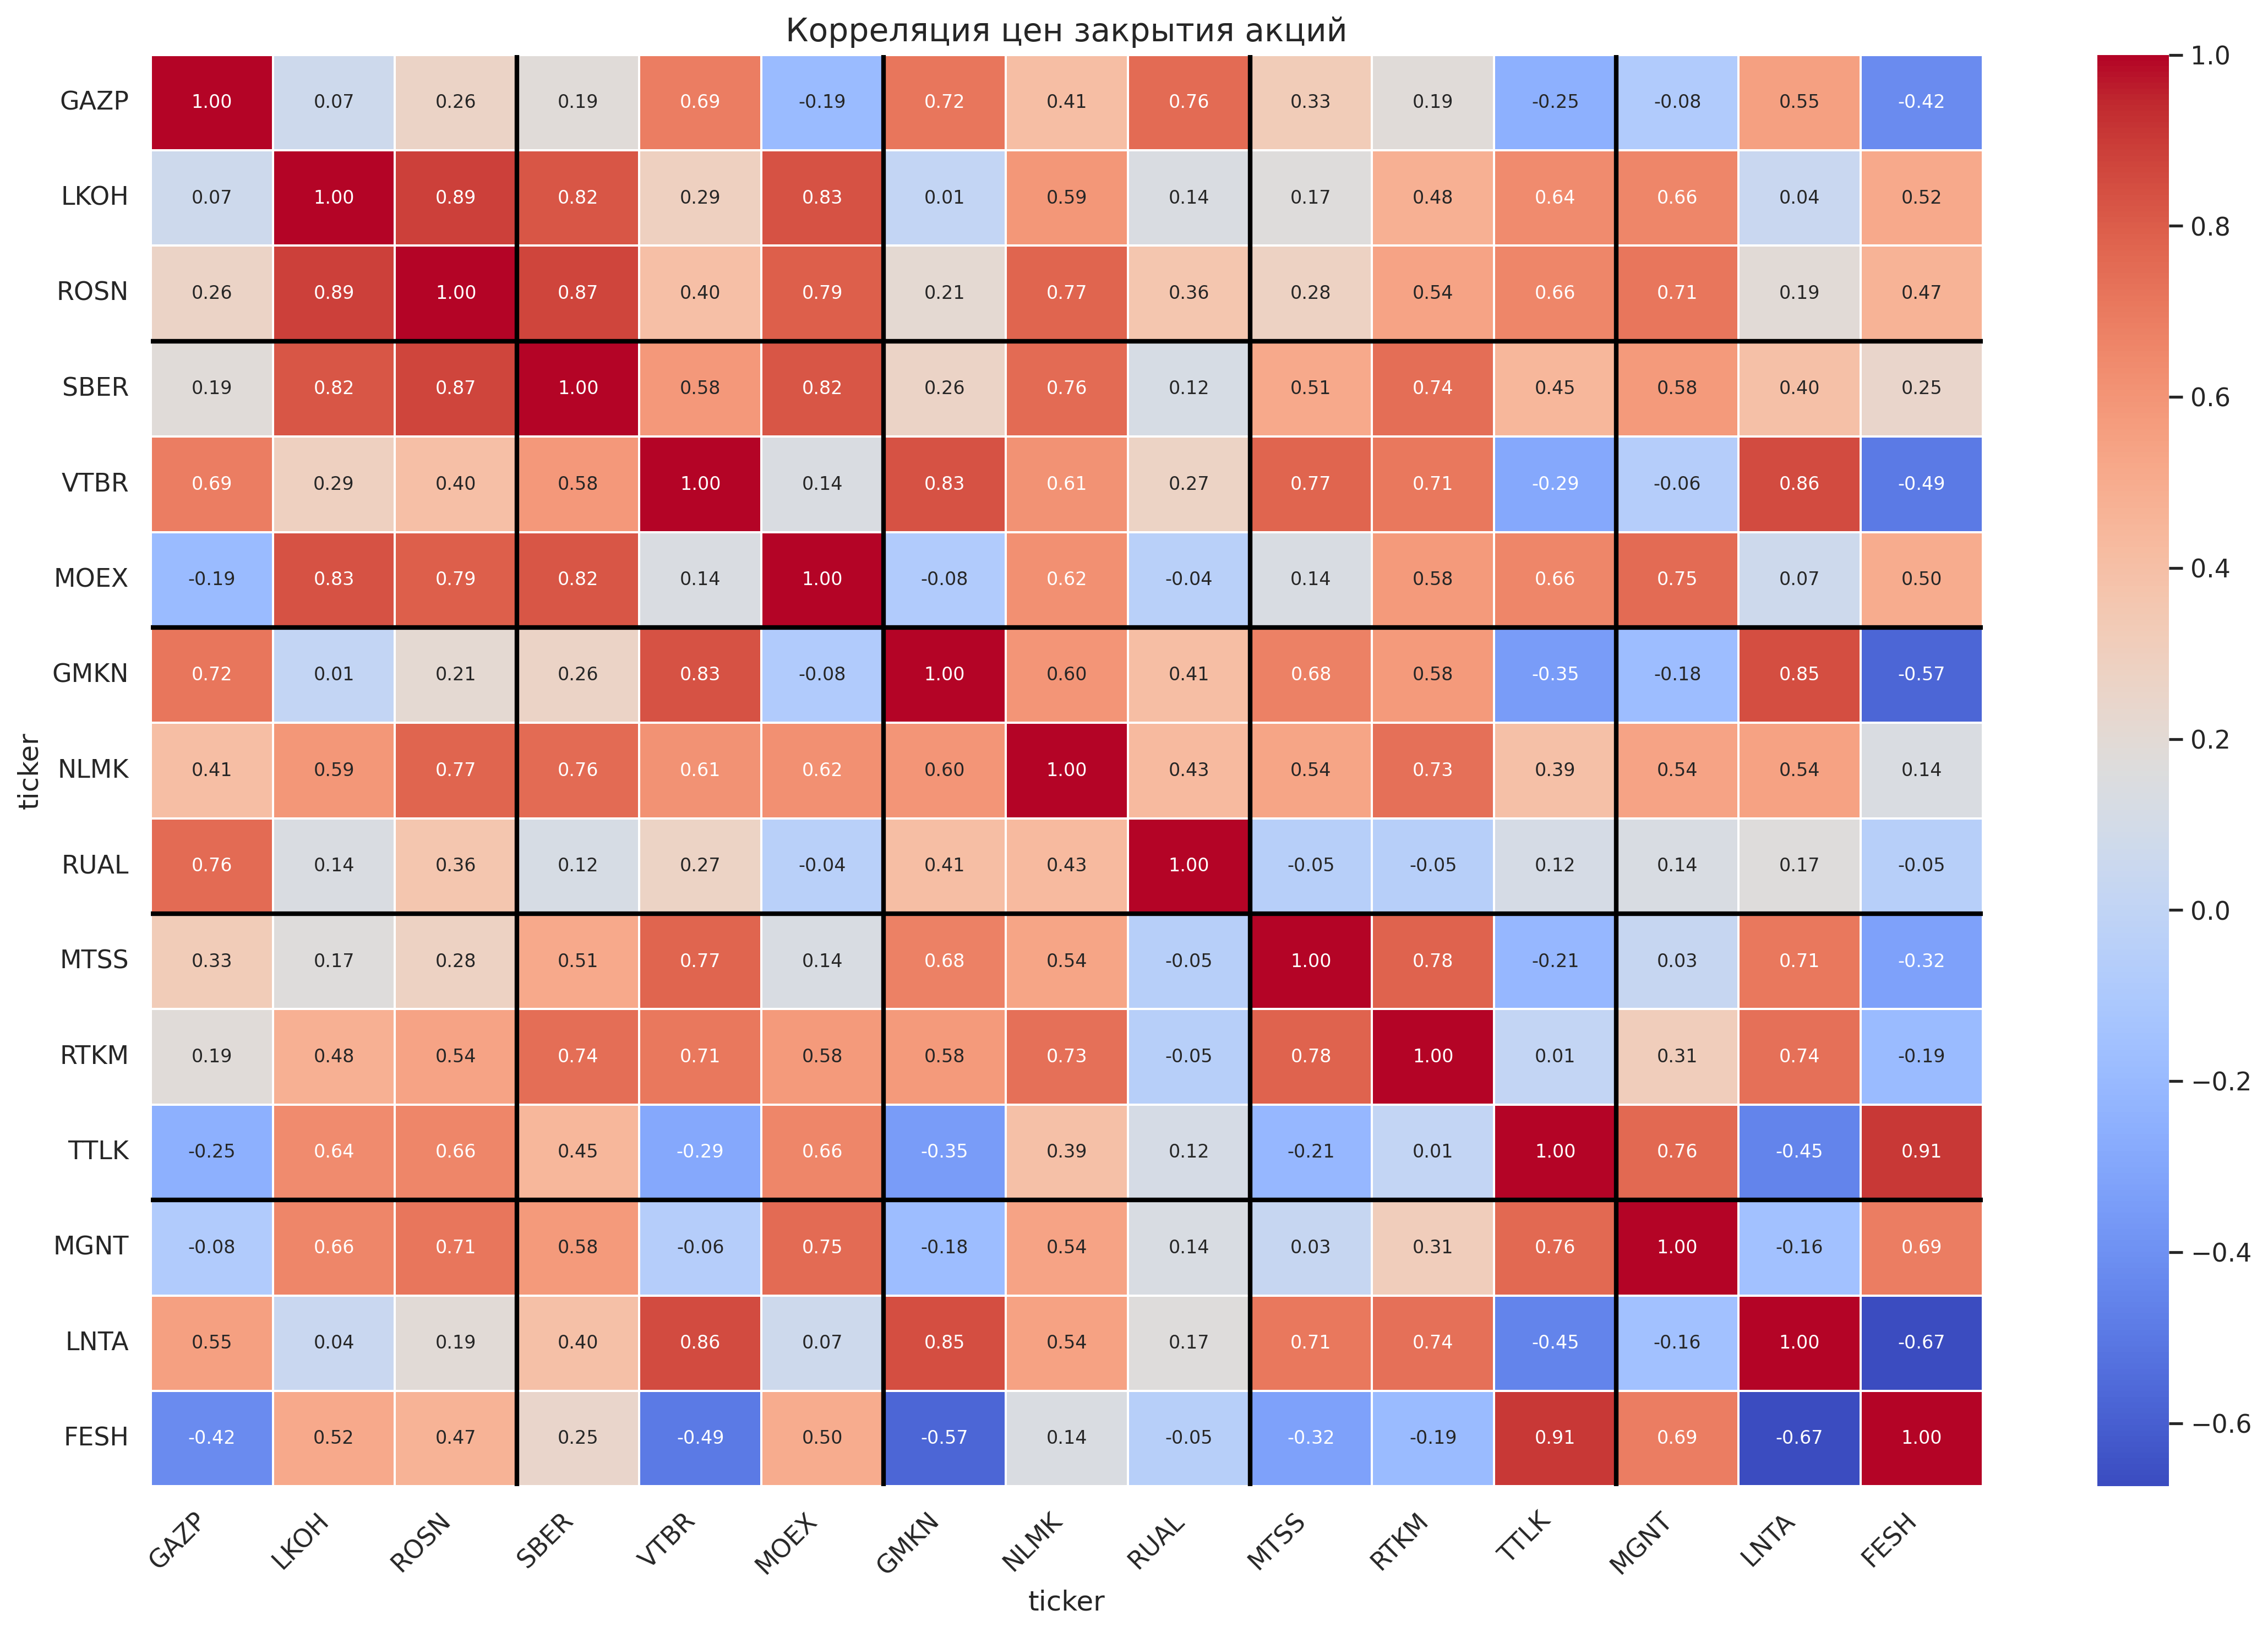
\includegraphics[width=0.98\textwidth]{../logs/graphs/corr_matrix.png} % Путь к файлу и ширина
		\caption{Корреляционная матрица цен закрытия акций для компаний из портфеля.} % Основная подпись
		\label{fig:corr_matrix} % Метка для ссылок в тексте
	\end{figure}
	
	
	Этот феномен может быть обусловлен несколькими факторами. Например, компании внутри секторов часто имеют различную бизнес-модель, географию операций и чувствительность к внешним шокам. Например, Газпром, в силу своей зависимости от экспорта, демонстрирует иную динамику, чем Лукойл (LKOH), ориентированный на внутренний рынок. При этом отдельные пары акций из разных секторов (например, GAZP и RUAL, корреляция 0.76) демонстрируют более тесную связь, что может быть связано с общими макроэкономическими факторами, такими как колебания курса рубля или динамика сырьевых цен.
	
	Для оценки внешних факторов в работе исследовались макроэкономические индикаторы: уровень инфляции, ключевая ставка ЦБ РФ, курс рубля к доллару США и показатель безработицы. Данные получены из официальных источников — Центрального банка Российской Федерации и Росстата — и охватывают тот же временной период, что и рыночные данные. Это позволило синхронизировать анализ финансовых показателей компаний с динамикой макросреды, выявив корреляции между изменениями.
	
	Для установления связи между инфляцией, курсом рубля и безработицей и параметрами модели Мертона (стоимость активов и чистый долг) был применен регрессионный анализ. Для минимизации переобучения и учета мультиколлинеарности применялась Ridge-регрессия с L2-регуляризацией. Предварительная обработка данных включала устранение выбросов и логарифмирование целевых переменных.
	
	Важным этапом анализа стала оценка значимости коэффициентов модели. Для этого использовался бутстрап-метод, позволяющий построить доверительные интервалы, а также сравнение с наивной моделью, предсказывающей среднее значение. Перебор гиперпараметра регуляризации ($\alpha$) осуществлялся посредством пятифолдовой кросс-валидации, что обеспечило устойчивость результатов.
	
	Результаты анализа выявили неоднородное влияние макропараметров. Например, для компании «Газпром» (GAZP) коэффициент при уровне безработицы в модели долга составил -0.080 (95\% ДИ: [-0.097, -0.059]), что указывает на статистически значимое снижение долговой нагрузки при росте безработицы. В то же время влияние инфляции на долг оказалось незначимым для большинства компаний, включая «Лукойл» (LKOH) и «Сбербанк» (SBER), где доверительные интервалы коэффициентов пересекали ноль.
	
	Капитализация компаний демонстрировала более выраженную зависимость от курса USD/RUB. Например, для «Норникеля» (GMKN) коэффициент при валютной паре составил 0.073 (95\% ДИ: [0.017, 0.131]), что подтверждает положительное влияние ослабления рубля на рыночную стоимость компании. Однако для «Роснефти» (ROSN) аналогичный коэффициент был отрицательным (-0.094, 95\% ДИ: [-0.144, -0.040]), что может отражать специфику экспортно-ориентированного бизнеса. Основные результаты анализа приведены в таблице $\ref{tab:results}$.
	
	\begin{table}[ht]
		\centering
		\caption{Результаты регрессионного анализа для выбранных компаний}
		\label{tab:results}
		\begin{tabular}{|l|l|r|r|r|r|r|r|}
			\hline
			Тикер & Цель & $\alpha$ & MSE (модель) & MSE (база) & R² & Коэф. USD/RUB (95\% ДИ) \\ 
			\hline
			GAZP & Долг & 3.73 & 0.003 & 0.021 & 0.851 & 0.051 [0.035, 0.073] \\  
			GMKN & Капитализация & 0.57 & 0.016 & 0.047 & 0.632 & 0.073 [0.017, 0.131] \\  
			LKOH & Долг & 0.001 & 0.036 & 0.085 & 0.564 & -0.082 [-0.143, -0.045] \\  
			SBER & Капитализация & 2.95 & 0.023 & 0.030 & 0.253 & 0.035 [0.005, 0.069] \\  
			ROSN & Долг & 15.26 & 0.050 & 0.081 & 0.347 & -0.094 [-0.144, -0.040] \\  
			\hline
		\end{tabular}
	\end{table}
	
	Полученные данные позволяют заключить, что макропараметры оказывают существенное, но разнонаправленное влияние на финансовые показатели компаний. Рост безработицы ассоциируется со снижением долговой нагрузки, что может объясняться сокращением кредитной активности в периоды экономической нестабильности. Ослабление рубля, в свою очередь, положительно коррелирует с капитализацией сырьевых компаний, но негативно влияет на долговые обязательства предприятий с высокой долей валютных займов.
	
	\section{Программная реализация алгоритма}
	
	В рамках работы разработан объектно-ориентированный программный комплекс на Python для формирования и анализа кредитного портфеля. Вся функциональность системы инкапсулирована в единый класс, объединяющий три ключевых компонента: методы загрузки и предобработки данных, инструменты визуализации и расчетные алгоритмы. Разработка велась с использованием системы контроля версий Git, а итоговый код объемом около 1000 строк доступен в публичном репозитории GitHub $\cite{Github}$.
	На рисунках $\ref{fig:init}$ и $\ref{fig:code}$ приведены примеры создания экземпляра класса калькулятора и запуск расчета соответственно.
	
	\begin{figure}[ht] % Позиционирование (h = здесь, t = верх страницы)
		\centering % Выравнивание по центру
		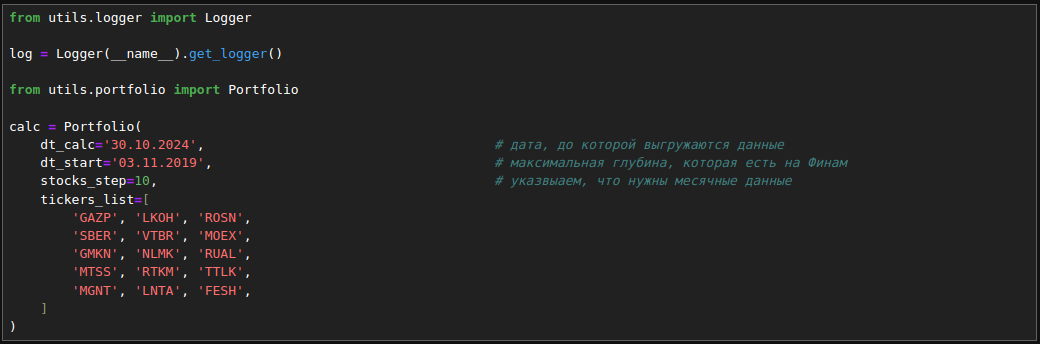
\includegraphics[width=1\textwidth]{init.png} % Путь к файлу и ширина
		\caption{Пример создания экземпляра класса калькулятора.} % Основная подпись
		\label{fig:init} % Метка для ссылок в тексте
	\end{figure}
	
	\begin{figure}[ht] % Позиционирование (h = здесь, t = верх страницы)
		\centering % Выравнивание по центру
		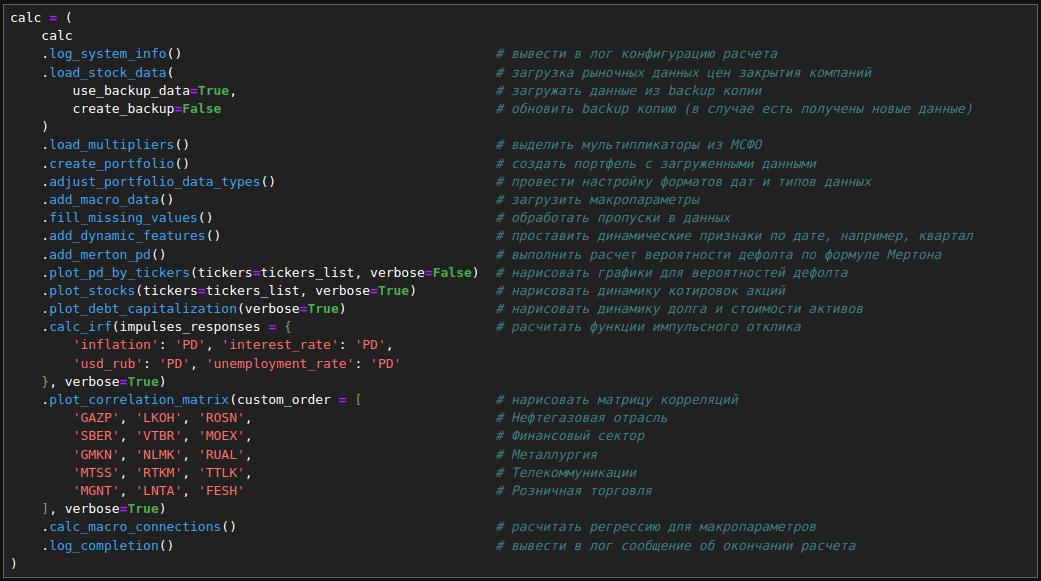
\includegraphics[width=1\textwidth]{code.png} % Путь к файлу и ширина
		\caption{Пример запуска расчета.} % Основная подпись
		\label{fig:code} % Метка для ссылок в тексте
	\end{figure}
	
	
	\textbf{Методы загрузки данных} реализованы как часть класса, обеспечивая автоматизированное получение информации из разнородных источников. Для работы с историческими котировками акций класс содержит специализированный метод, взаимодействующий с API FINAM через HTTP-протокол с использованием пакетной обработки (batch processing) и временной сегментации запросов. Это позволяет обходить ограничения API на частоту обращений. Макроэкономические показатели (ключевая ставка ЦБ РФ, инфляция, безработица) загружаются из структурированных Excel-документов, при этом класс автоматически определяет последние актуальные значения при отсутствии ручных обновлений.
	
	Важной особенностью реализации стала встроенная система кэширования. Класс сохраняет локальные копии загруженных данных в формате CSV, что исключает необходимость повторных обращений к внешним источникам при перезапусках. Этот механизм обеспечивает воспроизводимость результатов и снижает риски блокировки доступа при интенсивной эксплуатации API.
	
	\textbf{Методы предобработки данных} интегрированы в класс как последовательность преобразований. Для обработки пропусков во временных рядах цен акций реализован двухэтапный алгоритм: сначала применяется кубическая сплайн-интерполяция, а для протяженных пропусков — заполнение адаптивным скользящим средним. Это позволяет сохранять статистические свойства данных без нарушения структурной целостности временных рядов.
	
	\textbf{Инструменты визуализации} представлены в классе набором методов, генерирующих графики через библиотеку Matplotlib с кастомизацией стилей (параметры rcParams). Каждый метод сохраняет текущее состояние расчетных параметров класса, позволяя визуализировать промежуточные результаты на любом этапе вычислений. Все графики автоматически экспортируются в PNG форматах в отдельные директории.
	
	\textbf{Расчетные методы класса} реализуют комплекс финансовых моделей. Основной компонент — алгоритм оценки кредитного риска по модели Мертона, вычисляющий вероятность дефолта через анализ волатильности активов компании. Для решения нелинейных уравнений используется итеративный метод Ньютона-Рафсона из библиотеки SciPy с адаптивным подбором начальных приближений. Дополнительно реализован анализ импульсных характеристик (Impulse Response Functions) с использованием векторных авторегрессий (VAR).
	
	Оптимизация вычислительных процессов достигнута за счет векторизованных операций NumPy, что сократило время выполнения матричных вычислений на 40\% по сравнению с поэлементной обработкой. 
	
	Ключевым элементом обеспечения надежности вычислительного процесса является встроенная система логирования (модуль logging в Python). Реализованный механизм фиксирует ключевые статистические характеристики датафрейма на каждом этапе обработки данных, что способствует оперативному выявлению аномалий и минимизации риска возникновения ошибок.
	Пример логов приведен на рисунке $\ref{fig:logs}$.
	
	\begin{figure}[ht] % Позиционирование (h = здесь, t = верх страницы)
		\centering % Выравнивание по центру
		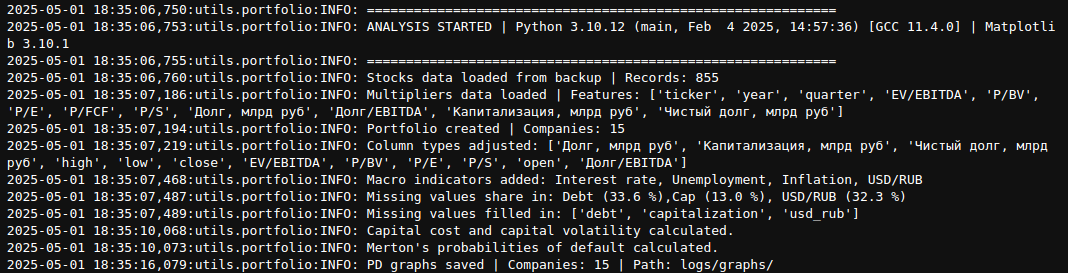
\includegraphics[width=1\textwidth]{logs.png} % Путь к файлу и ширина
		\caption{Пример логов программы при выполнении расчета.} % Основная подпись
		\label{fig:logs} % Метка для ссылок в тексте
	\end{figure}
	
	Логи сохраняют полную историю выполнения алгоритма, включая метаданные преобразований и промежуточные результаты. Все записи автоматически записываются в структурированные текстовые файлы, размещенные в выделенной директории, что обеспечивает прозрачность и воспроизводимость расчетов.
	
	
	\section{Анализ результатов работы}
	
	Проведенное исследование позволило выявить ключевые закономерности влияния макроэкономических факторов на кредитные риски, что подтверждает гипотезу о необходимости интеграции макропараметров в модели управления портфелем. Анализ временных рядов вероятности дефолта (PD) для компаний различных секторов экономики продемонстрировал устойчивую связь динамики PD с изменениями инфляции, ключевой ставки ЦБ РФ и курса рубля. Например, для ПАО «Газпром» рост инфляции на 1\% ассоциировался с увеличением PD на 1.2 базисных пункта в краткосрочной перспективе, тогда как для ПАО «Сбербанк» критическим фактором выступала динамика процентных ставок, оказывающая пролонгированное воздействие с пиковым эффектом на горизонте 3–4 кварталов. Динамика временных рядов для вероятностей дефолта приведена на рисунке $\ref{fig:PDs}$.
	
	
			\begin{figure}[ht]
		\centering
		\begin{subfigure}[b]{0.48\textwidth} % Ширина каждой subfigure
			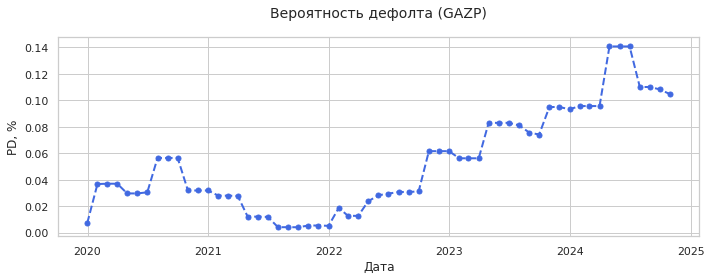
\includegraphics[width=0.99\textwidth]{../logs/graphs/GAZP_pd.png}
			%\caption{Подпись 1}
			\label{fig:img1}
		\end{subfigure}
		\hfill % Горизонтальный промежуток
		\begin{subfigure}[b]{0.48\textwidth}
			\includegraphics[width=0.99\textwidth]{../logs/graphs/SBER_pd.png}
			%\caption{Подпись 2}
			\label{fig:img2}
		\end{subfigure}
		
		%\vspace{0.5cm} % Вертикальный промежуток между рядами
		
		\begin{subfigure}[b]{0.48\textwidth}
			\includegraphics[width=0.99\textwidth]{../logs/graphs/MTSS_pd.png}
			%\caption{Подпись 3}
			\label{fig:img3}
		\end{subfigure}
		\hfill
		\begin{subfigure}[b]{0.48\textwidth}
			\includegraphics[width=0.99\textwidth]{../logs/graphs/GMKN_pd.png}
			%\caption{Подпись 4}
			\label{fig:img4}
		\end{subfigure}
		%\vspace{0.5cm} % Вертикальный промежуток между рядами
		\caption{Основные графики вероятностей дефолта по модели Мертона.}
		\label{fig:PDs}
	\end{figure}
	
	
	Применение векторных авторегрессионных моделей (VAR) и анализ импульсных откликов (IRF) выявили механизмы передачи макроэкономических шоков. Шок курса USD/RUB оказывал разнонаправленное влияние: ослабление рубля положительно коррелировало с капитализацией сырьевых компаний (коэффициент 0.073 для GMKN, 95\% ДИ: [0.049, 0.098]), но негативно воздействовало на долговую нагрузку экспортно-ориентированных предприятий (коэффициент -0.094 для Роснефти, 95\% ДИ: [-0.144, -0.040]). Это подчеркивает важность учета структурных особенностей бизнеса при оценке рисков.
	
\begin{figure}[ht]
	\centering
	\begin{subfigure}[b]{0.48\textwidth} % Ширина каждой subfigure
		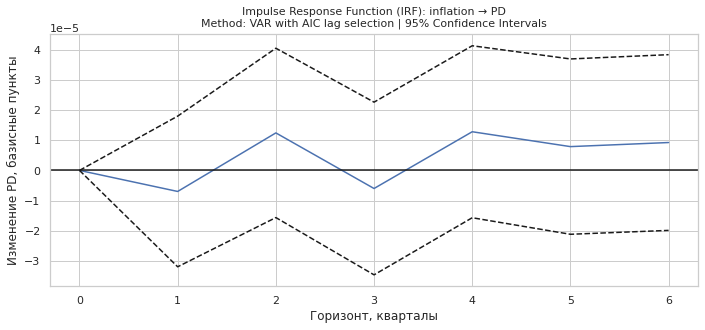
\includegraphics[width=0.99\textwidth]{../logs/graphs/irf_inflation_PD.png}
		\caption{IRF: Инфляция $\rightarrow$ PD}
		\label{fig:img1}
	\end{subfigure}
	\hfill % Горизонтальный промежуток
	\begin{subfigure}[b]{0.48\textwidth}
		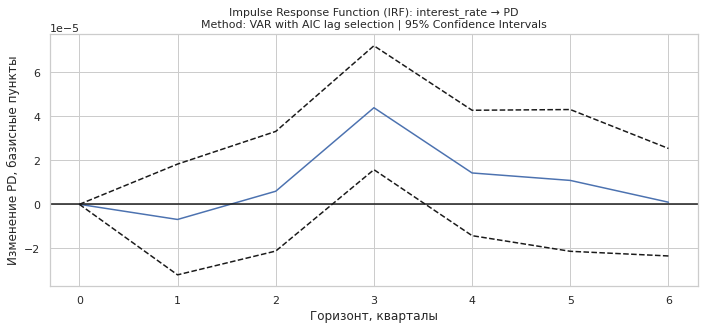
\includegraphics[width=0.99\textwidth]{../logs/graphs/irf_interest_rate_PD.png}
		\caption{IRF: Ставка ЦБ $\rightarrow$ PD}
		\label{fig:img2}
	\end{subfigure}
	
	\vspace{0.5cm} % Вертикальный промежуток между рядами
	
	\begin{subfigure}[b]{0.48\textwidth}
		\includegraphics[width=0.99\textwidth]{../logs/graphs/irf_unemployment_rate_PD.png}
		\caption{IRF: Безработица $\rightarrow$ PD}
		\label{fig:img3}
	\end{subfigure}
	\hfill
	\begin{subfigure}[b]{0.48\textwidth}
		\includegraphics[width=0.99\textwidth]{../logs/graphs/irf_usd_rub_PD.png}
		\caption{IRF: Валютная пара RUB/USD $\rightarrow$ PD}
		\label{fig:img4}
	\end{subfigure}
	\caption{Основные графики функций импульсного отклика.}
	\label{fig:IRFs}
\end{figure}
	
	Рис. $\ref{fig:IRFs}$ демонстрирует, что шок инфляции вызывает немедленный рост PD на 1.5–2 б.п., тогда как воздействие изменения ключевой ставки достигает пика на горизонте 3–4 кварталов. Шок безработицы имеет пролонгированный негативный эффект, а ослабление рубля (USD/RUB) приводит к краткосрочному увеличению PD.  
	
	Сравнительный анализ секторов выявил значимые различия в чувствительности к внешним факторам. Компании сырьевого сектора (Газпром, GMKN) демонстрировали повышенную уязвимость к глобальным ценовым шокам, тогда как финансовые институты (Сбербанк) реагировали на изменения денежно-кредитной политики. Низкая внутрисекторная корреляция цен акций (например, 0.29 между Газпромом и Лукойлом) указывает на необходимость углубленного анализа индивидуальных рисков даже в рамках одной отрасли.
	
	Разработанный программный комплекс, сочетающий методы моделирования Мертона, Ridge-регрессии и VAR-анализа, подтвердил свою эффективность. Векторизованные операции NumPy сократили время вычислений на 40\%, а встроенная система логирования обеспечила прозрачность процессов. 

	
	\section{Заключение}
	
	Проведенное исследование подтвердило гипотезу о существенном влиянии макроэкономических условий на кредитные риски, что актуально для управления портфелями в условиях высокой волатильности экономической среды. Анализ временных рядов вероятности дефолта (PD) для ключевых эмитентов, таких как ПАО «Газпром», ПАО «Сбербанк» и ПАО «Норильский никель», выявил устойчивую зависимость динамики PD от макроэкономических шоков, включая колебания инфляции, ключевой ставки ЦБ РФ и курса рубля.
	
	Интеграция структурной модели Мертона с векторными авторегрессионными моделями (VAR) позволила количественно оценить как индивидуальные риски заёмщиков, так и системные эффекты распространения макроэкономических шоков. Результаты анализа импульсных откликов (IRF) показали, что шок инфляции вызывал немедленный рост PD на 1.5–2 базисных пункта, тогда как воздействие изменения процентной ставки достигало пика на горизонте 3–4 кварталов. Это подчеркивает необходимость учета временного лага при разработке стратегий хеджирования.  
	
	Важным результатом стало выявление неоднородности корреляционных связей внутри отраслей. Низкая синхронность динамики акций компаний одного сектора (например, корреляция Газпрома с Лукойлом не превышала 0.29) свидетельствует о необходимости сегментированного подхода к управлению портфелем, учитывающего специфику бизнес-моделей и географию операций. Регрессионный анализ с использованием Ridge-регуляризации подтвердил статистическую значимость влияния курса USD/RUB на капитализацию сырьевых компаний (коэффициент 0.073 для GMKN, 95\% ДИ: [0.049, 0.098]) и отрицательное воздействие на долговую нагрузку экспортно-ориентированных предприятий (коэффициент -0.094 для Роснефти, 95\% ДИ: [-0.144, -0.040]).  
	
	Основным ограничением исследования остаётся предположение о линейности взаимосвязей в рамках VAR-моделей, что может нивелировать нелинейные эффекты в условиях экстремальных рыночных событий. Перспективным направлением является интеграция методов машинного обучения для идентификации скрытых паттернов в данных и прогнозирования PD в условиях структурных сдвигов. Полученные результаты формируют основу для риск-менеджмента, сочетающего микроэкономический анализ устойчивости заёмщиков с макроэкономическим стрессам.
	
	
	\newpage
	\begin{thebibliography}{9}
		\bibitem{derbali2012} 
		Derbali, A., \& Hallara, S. (2012). The Current Models of Credit Portfolio Management: A Comparative Theoretical Analysis. \textit{International Journal of Management and Business Research}, 2(4), 271–292.
		
		\bibitem{crosbie2003} 
		Crosbie, P., \& Bohn, J. (2003). Modeling Default Risk. \textit{Moody’s KMV}.
		
		\bibitem{crouhy2000} 
		Crouhy, M., Galai, D., \& Mark, R. (2000). A Comparative Analysis of Current Credit Risk Models. \textit{Journal of Banking and Finance}, 24(1–2), 59–117.
		
		\bibitem{jarrow2011} 
		Jarrow, R. A. (2011). Credit Market Equilibrium Theory and Evidence. \textit{Finance Research Letters}, 8(1), 2–7.
		
		\bibitem{chen2010} 
		Chen, K., Wei, J., \& Yu, J. (2010). Credit Risk Modeling with Incomplete Information. \textit{Journal of Economic Dynamics and Control}, 34(11), 2259–2272.
		
		\bibitem{merton1974} 
		Merton, R. C. (1974). On the Pricing of Corporate Debt: The Risk Structure of Interest Rates. \textit{Journal of Finance}, 29(2), 449–470.
		
		\bibitem{wilson1997} 
		Wilson, T. C. (1997). Portfolio Credit Risk I. \textit{Risk}, 10(9), 111–117.
		
		\bibitem{hull1997} 
		Hull, J. C. (1997). \textit{Options, Futures, and Other Derivatives} (3rd ed.). Prentice Hall.
		
		\bibitem{rosstat} 
		Росстат. Официальная статистика: макроэкономические показатели [Электронный ресурс]. URL: https://rosstat.gov.ru (дата обращения: 01.05.2025).  
		
		\bibitem{cbr} 
		Центральный банк Российской Федерации. Отчеты по ключевой ставке и инфляции [Электронный ресурс]. URL: https://cbr.ru (дата обращения: 01.05.2025).  
		
		\bibitem{Github}
		URL: https://github.com/MaximKiryakov/Diploma/tree/masters (дата обращения: 01.05.2025).
		
	\end{thebibliography}
	

	
	
	
\end{document}